\section{Costruzione del problema}\label{sec:problema}

Per lo svolgimento di questo progetto, sono stati analizzati dataset di 
dimensioni contenute, selezionando un massimo di $n$ asset distinti. Per ciascun 
asset \(i\), con \(1 \leq i \leq n\), è stato considerato l'intervallo temporale 
tra il 01/01/2016 e il 01/01/2020. Per ogni giorno \(t\) in questo intervallo 
\((0 \leq t \leq T)\), la performance di un asset è rappresentata dal suo prezzo di 
chiusura \(p_i^t\).


La prima informazione estratta da questo dataset consiste nell'elenco \(P\) dei 
prezzi correnti \(P_i\) degli asset considerati:

\begin{equation}\label{eqn:prezzo}
    P_i = p_i^t. 
\end{equation}

Inoltre, per ciascun asset, il rendimento \(r_i^t\) tra i giorni \(t-1\) e \(t\) 
può essere calcolato come:

\begin{equation}\label{eqn:rendimentoreale}
    r_i^t = \frac{p_i^t - p_i^{t-1}}{p_i^{t-1}}. 
\end{equation}

Grazie a questi rendimenti, è possibile definire il rendimento atteso di un asset 
come una stima ragionata della sua futura performance. Supponendo una distribuzione 
normale dei rendimenti, la media dei loro valori in ogni momento \(t\) nel set di 
osservazioni storiche è un buon stimatore del rendimento atteso. Pertanto, dato 
l'intero dataset storico, il rendimento atteso di ciascun asset \(\mu_i\) è calcolato come:

\begin{equation}\label{eqn:rendimentoatteso}
    \mu_i = E[r_i] = \frac{1}{T} \sum_{t=1}^T r_i^t. 
\end{equation}

Seguendo lo stesso principio, la varianza del rendimento di ciascun asset, $\sigma_{ij}$, e la 
covarianza tra i rendimenti di asset differenti nel corso delle serie storiche, $\sigma_i^2$, 
possono essere calcolate come segue:

\begin{equation}\label{eqn:varianza}
    \sigma_{ij} = E[(r_i - \mu_i)(r_j - \mu_j)] = \frac{1}{T-1} \sum_{t=1}^T (r_i^t - \mu_i)(r_j^t - \mu_j),
\end{equation}

\begin{equation}\label{eqn:covarianza}
    \sigma_i^2 = E[{(r_i - \mu_i)}^2] = \frac{1}{T-1} \sum_{t=1}^T {(r_i^t - \mu_i)}^2. 
\end{equation}

Un portafoglio è definito come un insieme di investimenti \(x_i\) (misurati come frazione 
del budget o del numero di unità allocate) per ciascun asset \(i\) del mercato. Pertanto, 
il portafoglio è composto da un vettore di numeri reali o interi con dimensioni pari al 
numero di asset considerati. 

Una strategia ottimale di allocazione del portafoglio punta 
a \textbf{massimizzare} il rendimento del portafoglio \(\mu^\top x\) \textbf{minimizzando} 
il rischio, definito come la varianza del portafoglio \(x^\top \Sigma x\), la cui 
radice quadrata rappresenta la volatilità del portafoglio. In questo caso, 
\(\mu\) è il vettore dei rendimenti medi per ciascun asset \(i\) calcolato con la 
Formula~\ref{eqn:rendimentoatteso}, 

\begin{equation}\label{eqn:matriceRendimentiAttesi}
    \mu =
    \begin{bmatrix}
    \mu_0 \\
    \mu_1 \\
    \vdots \\
    \mu_n
    \end{bmatrix},
\end{equation}

\(\Sigma\) è la matrice di covarianza calcolata con le Formule~\ref{eqn:varianza} 
e~\ref{eqn:covarianza}, 

\begin{equation}\label{eqn:matriceCovarianza}
    % \quad
    \Sigma =
    \begin{bmatrix}
    \sigma_0^2 & \sigma_{10} & \cdots & \sigma_{n0} \\
    \sigma_{01} & \sigma_1^2 & \cdots & \sigma_{n1} \\
    \vdots & \vdots & \ddots & \vdots \\
    \sigma_{0n} & \sigma_{1n} & \cdots & \sigma_n^2
    \end{bmatrix},
\end{equation}

e \(x\) è il vettore delle frazioni di budget allocate per ciascun asset. 

L'obiettivo di trovare un portafoglio ottimale consiste 
quindi nel trovare il vettore \(x\) che minimizza la funzione obiettivo seguente:

\begin{equation}\label{eqn:funzioneObiettivo}
    \mathcal{L}(x) = q x^\top \Sigma x - \mu^\top x,
\end{equation}

dove il parametro di avversione al rischio \(q\) esprime la propensione 
dell'investitore al rischio, i.e., un compromesso tra rischio e rendimento.


In uno scenario realistico, il budget disponibile \(B\) è fisso. Pertanto, il 
vincolo secondo cui la somma degli \(x_i\) deve essere pari a 1 è valido, e può essere 
espresso nel seguente modo: 
\begin{equation}\label{eqn:vincoloBudget}
    B = \sum_{i=1}^N x_i = 1.
\end{equation}

Di conseguenza, il problema può essere espresso come segue:

\begin{equation}\label{eqn:funzioneProblema}
    \min_x (q x^\top \Sigma x - \mu^\top x),
\end{equation}

dove:
\begin{itemize}
    \item $x \in \{0,1\}^n$ denota il vettore delle variabili decisionali binarie, 
        che indicano quali asset selezionare e quali no, identificati con $x_i = 1$ 
        e $x_i = 0$, rispettivamente;
    \item $\mu \in \mathbb{R}^n$ definisce i rendimenti attesi degli asset;
    \item $\Sigma \in \mathbb{R}^{n \times n}$ specifica le covarianze tra gli asset;
    \item $q > 0$ controlla l'avversione al rischio del decisore;
    \item $B$ denota il budget, ovvero il numero di asset da selezionare tra gli $n$ 
        disponibili.
\end{itemize}

Per poter risolvere il problema mediante algoritmi quantistici, è necessario formularlo 
senza vincoli espliciti. Per questo motivo, introduciamo un termine di penalità che 
favorisce le soluzioni in cui il numero di asset selezionati, i.e., il numero di $1$ 
nel vettore $x$, sia il più vicino possibile al budget $B$.

Il problema di ottimizzazione risulta quindi:
\begin{equation}\label{eqn:funzioneProblemaConVincolo}
    \min_x \left(qx^T\Sigma x - x\mu^T + {({1}^T x - B)}^2\right).
\end{equation}

Questa formulazione rappresenta un Quadratic Unconstrained Binary Optimization 
problem (QUBO), che può essere risolto utilizzando algoritmi di ottimizzazione 
quantistica basati sul principio variazionale, come il Variational Quantum Eigensolver 
(VQE) e il Quantum Approximate Optimization Algorithm (QAOA), i quali verranno
approfonditi nelle Sezioni~\ref{sec:vqe} e~\ref{sec:qaoa}, rispettivamente.


\paragraph{Perchè usare il Quantum Computing}
Nel contesto dell'ottimizzazione di portafoglio, l'analisi della complessità 
computazionale rivela differenze significative tra l'approccio classico e quello 
quantistico. Nel caso classico, il problema ricade nella classe dei problemi NP-hard, 
dove lo spazio delle soluzioni cresce esponenzialmente: per $n$ variabili binarie, 
abbiamo $2^n$ possibili soluzioni, mentre per $x$ variabili intere che variano da 
0 a $x_{\max}$, lo spazio delle soluzioni diventa $(x_{\max}+1)^x$. 
Per gestire questa complessità, sono stati sviluppati metodi euristici che però mostrano 
limitazioni pratiche, risultando efficaci solo per portafogli con pochi asset.

L'approccio quantistico, invece, sfrutta fenomeni quantistici fondamentali 
come l'interferenza e l'entanglement per eseguire computazioni all'interno della 
classe di complessità BQP (Bounded-error Quantum Polynomial). 
Questa classe di problemi richiede un tempo polinomiale per la risoluzione su un 
computer quantistico, ritornando una soluzione corretta con probabilità maggiore 
o uguale a $\frac{2}{3}$~\cite{buonaiuto2023best}.


\begin{figure}[h!]\label{fig:complessita}
    \centering
    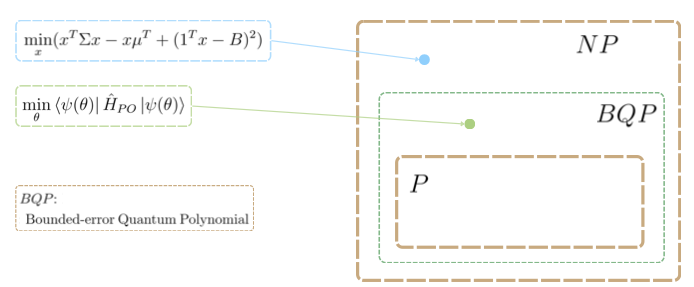
\includegraphics[width=0.8\textwidth]{images/complessita.png}
    \caption{Gerarchia delle classi di complessità computazionale.}
\end{figure}